\documentclass[a4paper]{article}
\usepackage{amsmath}
\usepackage{amsthm}
\usepackage[left=1.8cm,right=1.8cm,top=2.2cm,bottom=2.0cm]{geometry}
\usepackage{enumerate}
\usepackage{fancyhdr}
\usepackage{xpatch}
\usepackage{graphicx}
\usepackage{float}
\usepackage{subfigure}
\usepackage{amsfonts}
\usepackage{mathtools}
\usepackage{framed}
\usepackage{multicol}
\usepackage{fontspec}
\usepackage{float}
\usepackage{algpseudocode}
\usepackage{extarrows}
\usepackage{algorithm}
\usepackage{tikz}
\usepackage{caption}
\makeatletter

\printanswers


\AtBeginDocument{\xpatchcmd{\@thm}{\thm@headpunct{.}}{\thm@headpunct{}}{}{}}
\makeatother

\pagestyle{fancy}
\renewcommand{\baselinestretch}{1.15}
\newcommand{\code}[1]{\texttt{#1}}
\usepackage{paralist}
\let\itemize\compactitem
\let\enditemize\endcompactitem
\let\enumerate\compactenum
\let\endenumerate\endcompactenum
\let\description\compactdesc
\let\enddescription\endcompactdesc

% shorten footnote rule
\xpatchcmd\footnoterule
  {.4\columnwidth}
  {1in}
  {}{\fail}

\title{CSE 201: Homework 4}
% \author{\textbf{Yiwei Yang} \\ \texttt{ yyang363@ucsc.edu}}


\begin{document}
\maketitle
\section{Use Master Theorem to justify the following equation}
\subsection{  T(n) = √2 T(n/2) + log(n)}
We compare the given recurrence relation with $T(n)=a T(n / b)+\theta\left(n^k \log ^p n\right)$. $a=\sqrt{2}, b=2,k=0,p=1$. Now, $a = \sqrt{2}$ and $b^k = 2^0 = 1.$ $a>b^k$, thus $T(n)=\theta\left(n^{\log _b a}\right)=\theta\left(n^{\log _2 \sqrt{2}}\right)=\theta\left(n^{1 / 2}\right)$

\subsection{T(n) = 4 T(n/2) + n}
We compare the given recurrence relation with $T(n)=a T(n / b)+\theta\left(n^k \log ^p n\right)$. $a=4, b=2,k=1,p=0$. Now, $a = 4$ and $b^k = 2^1 = 2.$$a>b^k$, thus $T(n)=\theta\left(n^{\log _b a}\right)=\theta\left(n^{\log _2 4}\right)=\theta\left(n^{2}\right)$
  \subsection{T(n) = 2 T(n/2) + n log(n)}
  We compare the given recurrence relation with $T(n)=a T(n / b)+\theta\left(n^k \log ^p n\right)$. $a=2, b=2,k=1,p=1$. Since $p = 1$, so we have $T(n)=\theta\left(n^{\log _b a} \cdot \log ^{p+1} n\right)$
$S(n)=\theta\left(n^{\log _2 2} \cdot \log ^{1+1} n\right)$
$S(n)=\theta\left(n \cdot \log ^2 n\right)$
  \subsection{T(n) = 3 T(n/4) + n log(n)}
  We compare the given recurrence relation with $T(n)=a T(n / b)+\theta\left(n^k \log ^p n\right)$. $a=3, b=4,k=1,p=1$. Since $p=1$, so we have
$
T(n)=\theta\left(n^1 \log ^1 n\right)
T(n)=\theta\left(n \log  n\right)
$

  \section{Luke Skywalker}
  \begin{algorithm}
    \caption{Mod7Optimal$(x)$}\label{alg:cap1}
    \begin{algorithmic}[1]
      % \Require $n \geq 0$
      % \Ensure $y = x^n$
      \State{$rem=0$}
      \State{$i=0$}
      \While{$rem!=x$}
      \State $rem += (\lfloor \frac x {7^i}\rfloor \% 7)*7^i$
      \State $i=i+1$
      \EndWhile
    \end{algorithmic}
  \end{algorithm}
  The above algorithm is the optimal algorithm in terms of complexity, then we use the decision tree to deduce the complexity.
  \begin{center}
    \tikzset{every picture/.style={line width=0.75pt}} %set default line width to 0.75pt        
    \label{alg:cap}
    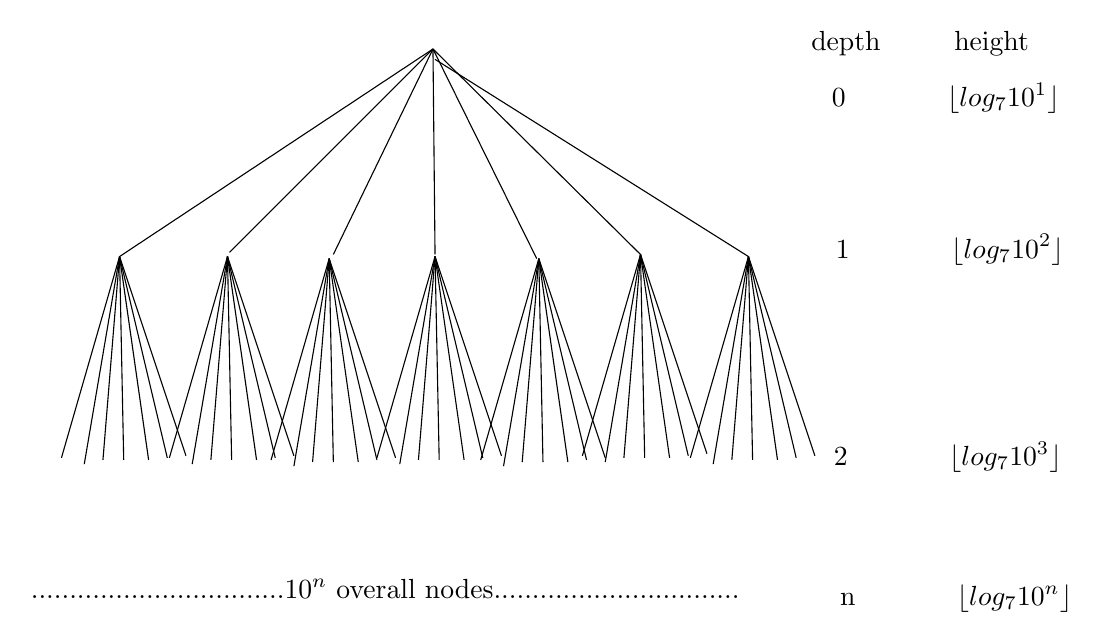
\begin{tikzpicture}[x=0.75pt,y=0.75pt,yscale=-1,xscale=1]
      %uncomment if require: \path (0,657); %set diagram left start at 0, and has height of 657

      %Straight Lines [id:da13708785911944021] 
      \draw    (349,51) -- (198,151) ;
      %Straight Lines [id:da8177036908727702] 
      \draw    (349,51) -- (251,149) ;
      %Straight Lines [id:da013465278431305405] 
      \draw    (349,51) -- (301,150) ;
      %Straight Lines [id:da21956955365509367] 
      \draw    (349,51) -- (350,150) ;
      %Straight Lines [id:da4757056545932208] 
      \draw    (349,51) -- (399,152) ;
      %Straight Lines [id:da4688062937675408] 
      \draw    (349,51) -- (449,150) ;
      %Straight Lines [id:da20664050669083434] 
      \draw    (350,56) -- (501,151) ;
      %Straight Lines [id:da1527456548058459] 
      \draw    (198,151) -- (170,248) ;
      %Straight Lines [id:da9969832807663619] 
      \draw    (198,151) -- (181,251) ;
      %Straight Lines [id:da831869369760321] 
      \draw    (198,151) -- (190,249) ;
      %Straight Lines [id:da8989901309451904] 
      \draw    (198,151) -- (200,249) ;
      %Straight Lines [id:da06422616663697456] 
      \draw    (198,151) -- (212,249) ;
      %Straight Lines [id:da008313412060936498] 
      \draw    (198,151) -- (221,248) ;
      %Straight Lines [id:da07238888780181085] 
      \draw    (198,151) -- (230,247) ;
      %Straight Lines [id:da4435950970068736] 
      \draw    (250,151) -- (222,248) ;
      %Straight Lines [id:da6992555511362868] 
      \draw    (250,151) -- (233,251) ;
      %Straight Lines [id:da5146768503577082] 
      \draw    (250,151) -- (242,249) ;
      %Straight Lines [id:da8126244399673677] 
      \draw    (250,151) -- (252,249) ;
      %Straight Lines [id:da10234085190097764] 
      \draw    (250,151) -- (264,249) ;
      %Straight Lines [id:da8540597039262281] 
      \draw    (250,151) -- (273,248) ;
      %Straight Lines [id:da534762654669964] 
      \draw    (250,151) -- (282,247) ;
      %Straight Lines [id:da9939885941343853] 
      \draw    (299,152) -- (271,249) ;
      %Straight Lines [id:da01869838794195533] 
      \draw    (299,152) -- (282,252) ;
      %Straight Lines [id:da1940667382755623] 
      \draw    (299,152) -- (291,250) ;
      %Straight Lines [id:da31445662952149434] 
      \draw    (299,152) -- (301,250) ;
      %Straight Lines [id:da7777818023221568] 
      \draw    (299,152) -- (313,250) ;
      %Straight Lines [id:da2053600116900982] 
      \draw    (299,152) -- (322,249) ;
      %Straight Lines [id:da31830711799948475] 
      \draw    (299,152) -- (331,248) ;
      %Straight Lines [id:da8960176112881433] 
      \draw    (350,151) -- (322,248) ;
      %Straight Lines [id:da7569507909250219] 
      \draw    (350,151) -- (333,251) ;
      %Straight Lines [id:da026488796984308616] 
      \draw    (350,151) -- (342,249) ;
      %Straight Lines [id:da6557280276280715] 
      \draw    (350,151) -- (352,249) ;
      %Straight Lines [id:da2311478379249583] 
      \draw    (350,151) -- (364,249) ;
      %Straight Lines [id:da25331507444255563] 
      \draw    (350,151) -- (373,248) ;
      %Straight Lines [id:da604265913958149] 
      \draw    (350,151) -- (382,247) ;
      %Straight Lines [id:da5760676008961665] 
      \draw    (400,152) -- (372,249) ;
      %Straight Lines [id:da7858199779356743] 
      \draw    (400,152) -- (383,252) ;
      %Straight Lines [id:da25675977576152476] 
      \draw    (400,152) -- (392,250) ;
      %Straight Lines [id:da528814442427318] 
      \draw    (400,152) -- (402,250) ;
      %Straight Lines [id:da24632215212833275] 
      \draw    (400,152) -- (414,250) ;
      %Straight Lines [id:da013672677768714614] 
      \draw    (400,152) -- (423,249) ;
      %Straight Lines [id:da9256843107127777] 
      \draw    (400,152) -- (432,248) ;
      %Straight Lines [id:da8799244231693513] 
      \draw    (449,150) -- (421,247) ;
      %Straight Lines [id:da24842050026090035] 
      \draw    (449,150) -- (432,250) ;
      %Straight Lines [id:da9893589185595129] 
      \draw    (449,150) -- (441,248) ;
      %Straight Lines [id:da1306282150006033] 
      \draw    (449,150) -- (451,248) ;
      %Straight Lines [id:da10725435952748863] 
      \draw    (449,150) -- (463,248) ;
      %Straight Lines [id:da17265726170175366] 
      \draw    (449,150) -- (472,247) ;
      %Straight Lines [id:da5923637900914207] 
      \draw    (449,150) -- (481,246) ;
      %Straight Lines [id:da9408036821091348] 
      \draw    (501,151) -- (473,248) ;
      %Straight Lines [id:da49780763315678467] 
      \draw    (501,151) -- (484,251) ;
      %Straight Lines [id:da5008124185799931] 
      \draw    (501,151) -- (493,249) ;
      %Straight Lines [id:da9654456416071875] 
      \draw    (501,151) -- (503,249) ;
      %Straight Lines [id:da5529746984207711] 
      \draw    (501,151) -- (515,249) ;
      %Straight Lines [id:da4130369513663559] 
      \draw    (501,151) -- (524,248) ;
      %Straight Lines [id:da7996306608104042] 
      \draw    (501,151) -- (533,247) ;


      % Text Node
      \draw (154,305) node [anchor=north west][inner sep=0.75pt]   [align=left] {.................................$\displaystyle 10^{n}$ overall nodes................................};
      % Text Node
      \draw (530,41) node [anchor=north west][inner sep=0.75pt]   [align=left] {depth \ \ \ \ \ \ \ height};
      % Text Node
      \draw (533,139) node [anchor=north west][inner sep=0.75pt]   [align=left] { \ \ 1 \ \ \ \ \ \ \ \ \ \ $\displaystyle \lfloor log_{7} 10^{2} \rfloor $ };
      % Text Node
      \draw (531,66) node [anchor=north west][inner sep=0.75pt]   [align=left] { \ \ 0 \ \ \ \ \ \ \ \ \ \ $\displaystyle \lfloor log_{7} 10^{1} \rfloor $ };
      % Text Node
      \draw (532,239) node [anchor=north west][inner sep=0.75pt]   [align=left] { \ \ 2 \ \ \ \ \ \ \ \ \ \ $\displaystyle \lfloor log_{7} 10^{3} \rfloor $ };
      % Text Node
      \draw (535,308) node [anchor=north west][inner sep=0.75pt]   [align=left] { \ \ n \ \ \ \ \ \ \ \ \ \ $\displaystyle \lfloor log_{7} 10^{n} \rfloor $ };


    \end{tikzpicture}
  \end{center}
  For every layer, the overall node number is the $n^10$, because everytime we can ask the 7-way question so that we can devide the space into 7 sets and for every set following we continuously goes to the last when we can get the anwer within 7. We recover the number by adding every bit of n digit of 7 with the remainders. By the property of the decision tree, the time complexity of any algorithm should compliance the height of this tree, which is $\Omega(\lfloor log_7 10^n\rfloor)=\Omega(n)$

\section{Median of two sorted array}
\subsection{Write pseudocode for an O(lg n) algorithm }
\begin{algorithm}
  \caption{MedianOfThree$(a,b,c)$}\label{alg:cap3}
  \begin{algorithmic}[1]
   \State {return $a + b + c - max(a, max(b, c)) - min(a, min(b, c))$}
  \end{algorithmic}
\end{algorithm}
\begin{algorithm}
  \caption{MedianOfFour$(a,b,c)$}\label{alg:cap4}
  \begin{algorithmic}[1]
    \State{$Max = max( a, max( b, max( c, d ) ) )$}
    \State{$Min = min( a, min( b, min( c, d ) ) )$}
    \State{return $\frac{ a + b + c + d - Max - Min }  2$}
  \end{algorithmic}
\end{algorithm}
The main algorithm is located Algorithm \ref{alg:cap2}.
\begin{algorithm}
  \caption{FindMedianOfTwoSortedArray$(A,n,B,m)$}\label{alg:cap2}
  \begin{algorithmic}[1]
    \If {$n>m$}
    \State{swap A,B}
    \State{swap m,n}
    \EndIf
    \If {$n=0$}
    \If {$m=0$}
    \State{return -1}
    \EndIf
    \If {$m \% 2 == 0$}
    \State{return $\frac{B[\frac {m} {2} ] + B[\frac {m}  {2} - 1] } {2}$}
    \EndIf
    \State{return $B[\frac {m-1} 2]$}
    \EndIf
    \If {$n=1$}
    \If {$m=1$}
    return $\frac{A[0]+ B[0]}2$
    \EndIf
    \If {$m \& 1 != 0$}
    \State{return $\frac{B[\frac{m}{2}] + MedianOfThree(A[0], B[\frac{m}{2} - 1], B[\frac{m}{2} + 1])}2$ }
    \EndIf
    \State{return $MedianOfFour (B[\frac{m}{2}], B[\frac{m}{2} - 1], max( A[0], B[\frac{m}{2} - 2] ), min( A[1], B[\frac{m}{2} + 1] ))$ }
    \Else
    \If{$n=2$}
    \If {$m =2$}
    \State{return $MedianOfFour(A[0], A[1], B[0], B[1])$}
    \EndIf
    \If {$m \& 1 != 0$}
    \State {return $MedianOfThree (B[\frac{m}{2}], max(A[0], B[\frac{m}{2} - 1]), min(A[1], B[\frac{m}{2} + 1])$)}
    \EndIf

    \State{return $MedianOfFour (B[\frac{m}{2}], B[\frac{m}{2} - 1], max( A[0], B[\frac{m}{2} - 2] ), min( A[1], B[\frac{m}{2} + 1] ))$}
    \Else
    \State{$idxA = \lfloor\frac{n - 1 }  2\rfloor$}
    \State{$idxB =  \lfloor\frac{m - 1 }  2\rfloor$}

    \If {$A[idxA] \leq B[idxB] $}
    \State{return $FindMedianOfTwoSortedArray(A + idxA, \frac n 2 + 1, B, m - idxA )$}
    \EndIf
    \State{return $FindMedianOfTwoSortedArray(A, \frac n 2 + 1, B + idxA, m - idxA )$}
    \EndIf
    \EndIf
  \end{algorithmic}
\end{algorithm}

\subsection{ Justify O(lg n)}
It is simple to observe that the binary search in the $A[1..n]$ range dominates the algorithm's complexity. We first make sure the B is always the bigger. With the base case $n=0,m=2k+1,k>1$ return B's median, just return $B[\frac{m-1}2]$, $n=0,m=2k,k>0$, also return B's median, this time is the median of middle 2 number. For base case $n=1, m=1$,just return median of 2 element in each array. For case $n=1,m=2k+1,k>1$, just return $\frac{B[\frac{m}{2}] + MedianOfThree(A[0], B[\frac{m}{2} - 1], B[\frac{m}{2} + 1])}2$. For case $n=1,m=2k,k>1$, we get $MedianOfFour (B[\frac{m}{2}], B[\frac{m}{2} - 1], max( A[0], B[\frac{m}{2} - 2] ), min( A[1], B[\frac{m}{2} + 1] ))$. For base case $n=2$, we have if $m=2$, we get $MedianOfFour(A[0],A[1],B[0],B[1])$, if $m=2k+1,k>1$, we get $MedianOfThree (B[\frac{m}{2}], max(A[0], B[\frac{m}{2} - 1]), min(A[1], B[\frac{m}{2} + 1])$, if $m=2k,k>1$, we have $MedianOfThree (B[\frac{m}{2}], max(A[0], B[\frac{m}{2} - 1]), min(A[1], B[\frac{m}{2} + 1])$. As a result of BST's back ward induction, the method executes in just $O(log\ m)$ time for getting the height of BST is $O(log\ m)$, and all of the solution conditions are verified simultaneously. The input vectors are labeled, though, making the $A$ array the smaller array. Therefore, the time complexity is merely for two randomly sorted arrays:
$$
O\left(\log \left(\min \left\{m, n\right\}\right)\right) 
$$
A similar temporal complexity of $O(log\text{ min }(m, n))$ applies to the merge-sort map's implementation of the median of two sorted arrays. This signifies that we were able to solve the issue more effectively.

\section{Maximal Increasing Subsequence problem}
\subsection{Optimal Subsequence}
Let $dp[m][n]$ be the Maximal Increasing Subsequence(MLS) from $arr[m]$ to $arr[n]$, say $n>m$

The Optimal Subsequence is, for j in 0..m, i in 0..n
$$dp[i][j]=\left\{\begin{array}{l}
  dp[i][j] = 0, \text{ when } i == 0 || j == 0\\
  dp[i][j] = 1 + dp[i - 1][j - 1], \text{ when } arr[j - 1] == arr[i - 1]\\
  dp[i][j] = max(dp[i - 1][j], dp[i][j - 1])
}\end{array}\right.$$
\subsection{Use Recurrence to solve this problem}
We can first define the optimal substructure, let M[i] be the input of teh length of the MIS ending at index i s.t. arr[i] is the last element of the MIS.

Thus, we can get the Recurrence function 
$$M[i]=\left\{\begin{array}{l}
 1+ max(M[j]), \text{ for } 0<j<i \text{ and } arr[j]<arr[i]\\
 1, \text{ else }
}\end{array}\right.$$

\begin{algorithm}
  \caption{MISRecursion$(arr,n)$}\label{alg:cap3}
  \begin{algorithmic}[1]
    \If{$n=1$}
      \State{return $1$}
    \EndIf
    \State{global $max\_ref$, initialize with 1}
    \State{initialize $res$ and $max\_ending$ with 1}
    \For{$i=1..n$}
    \State{$res=MISRecursion(arr,i)$}
    \If{$arr[i-1]<arr[j-1]\ \&\&\ res +1>max\_ending$}
      \State{$max\_ending = res+1$}
    \EndIf
    \EndFor
    \If{$max\_ref<max\_ending$}
     \State{$max\_ref=max\_ending$}
    \EndIf
    \State{return $max\_ending$}
  \end{algorithmic}
\end{algorithm}
\begin{proof}
  We proof by the forward induction. $arr[i]$ is the length of the MIS of the input until index $i$(including $i$), With every loop, we have already proved the stored $max\_ending$ is the maximal increasing subsequence that ends at any location. This is also assured when updating the global variable $max\_ref$ to assure the maximal history function calls.

  \textbf{Base Case:} $arr$ has only one element, returns 1, becaues it's the subsequence of itself.

  \textbf{Inductive Case:} Suppose the prior comparison of $res$ and $max\_ending$ are correct, we starts form $i$, the possible subsequence is arr[i] itself, whihc has length 1, the other possiblity is a subsequence that starts earlier and ends at $res$, and only occurs when $res>max\_ending$, and we need to set the $max\_ending=res+1$ to append the element res, which is the previous 1..i's biggest sub increasing sequence number.

  If the arr[i] is correct, the all algorithm is correct because it will continue to n.
\end{proof}
\subsection{Pseudocode}
\begin{algorithm}
  \caption{MISDP$(arr,n)$}
  \begin{algorithmic}[1]
  \State{initialize list b with sorted arr}
  \State{initialize m with b's len}
  \State{initialize dp[m+1][n+1]}
  \For {$i$ in $0..n+1$}
  \For {$j$ in $0..m+1$}
    \If{$i=0\text{ or }j=1$}
    \State{$dp[i][j]=0$}
    \Else \If{$a[i-1]=b[j-1]$}
    \State{$dp[i][j]=1+dp[i-1][j-1]$}
    \Else
    \State{$dp[i][j] = max(dp[i-1][j], dp[i][j-1])$}
    \EndIf
    \EndIf
  \EndFor
  \EndFor
  \State{return $dp[-1][-1]$}
  \end{algorithmic}
\end{algorithm}

\section{Greedy algorithm for shipping water}
\subsection{Pseudocode}
\begin{algorithm}
  \caption{ShipWater$(stop\_list,m)$}
  \begin{algorithmic}[1]
    \State{initialize $len$ with $len(stop\_list)$}
    \State{initialize $res$ with 0}
  \For {i in 0..n}
    \State{$curr\_num=0$}
    \For {j in i..n}
    \State{$curr\_num+=stop\_list[j]$}
    \If{$curr\_num>m$}
      \State{$refill\_water()$}
      \State{$res+=1$}
      \State{$i=j-1$}
      \Break
    \EndIf
    \EndFor
  \EndFor
  \EndFor
  \State{return $res$}
  \end{algorithmic}
\end{algorithm}
The $stop\_list$ inserted is the list of distance between each 2 stops. and m is each time how much one quater of water can Prof. Johnson bring.

\subsection{Correctness}
\begin{proof}
We prove by induction that after $res$ stops are passed. As a base case, after 1 stops are added, $curr\_num$ is $stop\_list[0]$ and $stop\_list$ remains the same.

For the inductive step, assume the claim is true after $res$ stops are passed. If at this point we have the rest of $curr\_num$ exactly can fit within the $m$, the algorithm terminates. Otherwise, updated $curr\_num \geq m$, so the algorithm proceeds for another iteration. We need to stop the stop before last $j$. update $i=j-1$, everything comes again.

The greedy calculation of the $curr\_num$ can proceed to the end, thus it's correct at the end.
\end{proof}
\subsection{Running Time}
It will take $O(n)$ because the worst case is every time it will loop only once for $i$, and the inner loop will take $O(n-i+i)$, thus the time complexity is $O(n*n)=O(n)$
\end{document}
